%----------------------------------------------------------------------------
\label{absorption data section}
%----------------------------------------------------------------------------
%----------------------------------------------------------------------------
%bb defines the bounding box for the pdf
%viewport defines the area of the pdf used
%in sidewaysfigure the last entry in bb moves the caption toward/away the pic
%in sidewaysfigure the second entry in bb moves the pic toward/away the caption
%----------------------------------------------------------------------------
\begin{figure}
\scalebox{0.8}[0.8]{
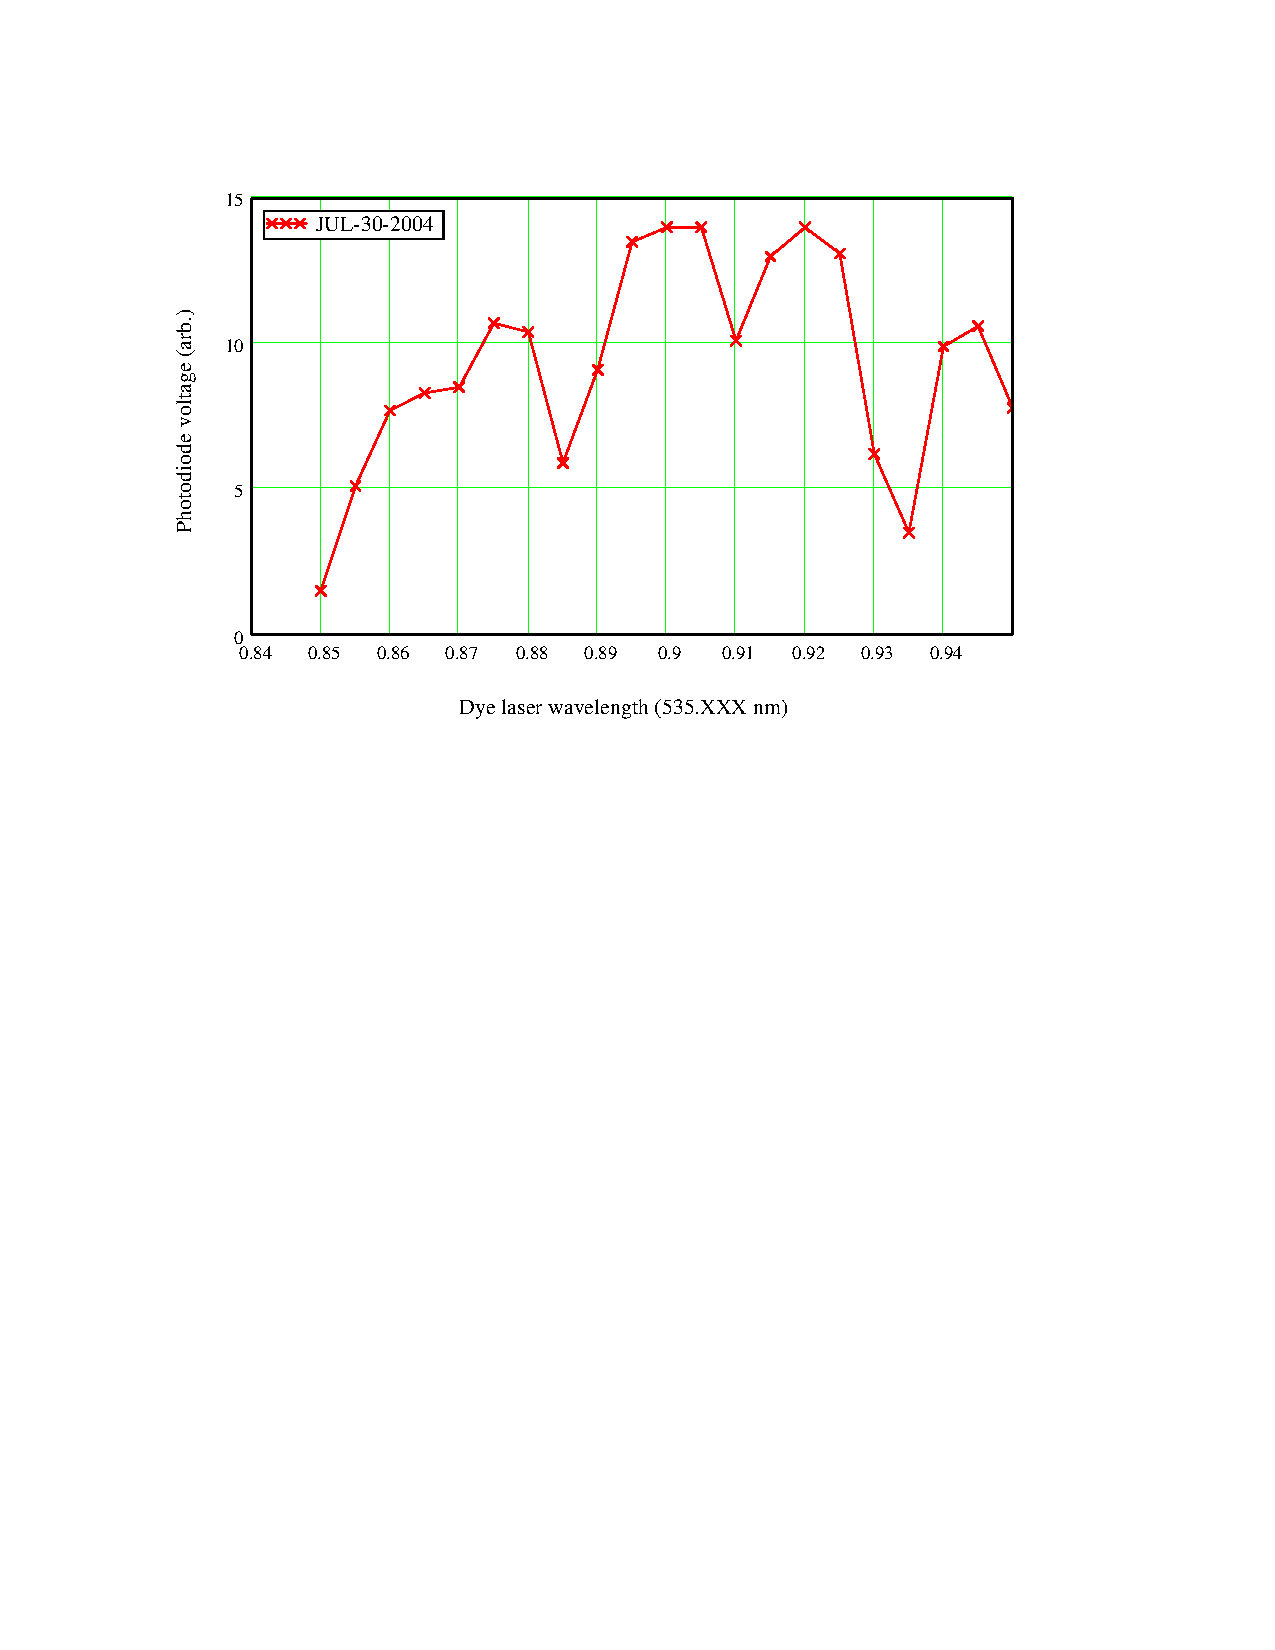
\includegraphics[bb=20 450 489 700]
{absorption/absorption.pdf}
}
\caption[Iodine absorption dye laser scan]{Iodine absorption dye laser scan. The fluctuations  were about $\pm20$\% of the value on the vertical scale (see UH notebook UH-016 page 9).}
\label{absorption}
\end{figure}
%----------------------------------------------------------------------------

%----------------------------------------------------------------------------
The output of the boxcar averager is connected to the vertical axis of a chart recorder. At each ``lambdalok'' setting the vertical position of the pen is recorded after the boxcar output stabilizes (the experimental repetition rate is 20 Hz and the ``samples'' setting on the averager is set to 300). See Figure \ref{absorption} for a plot of these data. The absorption peak (the ``peak'' points down) near 535.885 nm is the focus of the following discussion.

There are two transitions under investigation in this study. The first is the transition between the $\nu^{\prime\prime}=0$, $J^{\prime\prime}=52$ state in the X band to the $\nu^{\prime}=30$, $J^{\prime}=51$ state in the B band, called ``transition one'' hereafter. The second is the transition between the $\nu^{\prime\prime}=0$, $J^{\prime\prime}=55$ state in the X band to the $\nu^{\prime}=30$, $J^{\prime}=56$ state in the B band, called ``transition two'' hereafter.

Transition one has an excitation energy corresponding to 535.8843 nm while transition two has an excitation energy corresponding to 535.8901 nm. The resolution of the scan is high enough to identify the absorption feature associated with these transitions; however, the individual transitions are not resolved and may indeed prove difficult to resolve with this scanning method. The goal of this exercise was not to identify specific peaks; instead, we simply seek to verify the performance of the dye lasers (again, it is discovered the ``scan'' feature was unreliable) and observe the basic absorption features of molecular iodine.

%----------------------------------------------------------------------------
%----------------------------------------------------------------------------
%----------------------------------------------------------------------------
%----------------------------------------------------------------------------
%----------------------------------------------------------------------------
%----------------------------------------------------------------------------
